\documentclass[conference]{IEEEtran}
\IEEEoverridecommandlockouts
% The preceding line is only needed to identify funding in the first footnote. If that is unneeded, please comment it out.
\usepackage{cite}
\usepackage{amsmath,amssymb,amsfonts}
\usepackage{algorithmic}
\usepackage{graphicx}
\usepackage{textcomp}
\usepackage{xcolor}
\usepackage[brazilian]{babel}
\usepackage[utf8]{inputenc}
\usepackage[T1]{fontenc}
\usepackage{listings}
\usepackage{listings-golang}
\usepackage{color}
\usepackage{float}
\usepackage{multirow}
\usepackage{hyperref}

\definecolor{dkgreen}{rgb}{0,0.6,0}
\definecolor{gray}{rgb}{0.5,0.5,0.5}
\definecolor{mauve}{rgb}{0.58,0,0.82}

\lstset{frame=tb,
  language=Golang,
  aboveskip=3mm,
  belowskip=3mm,
  showstringspaces=false,
  columns=flexible,
  basicstyle={\small\ttfamily},
  numbers=none,
  numberstyle=\tiny\color{gray},
  keywordstyle=\color{blue},
  commentstyle=\color{dkgreen},
  stringstyle=\color{mauve},
  breaklines=true,
  breakatwhitespace=true,
  tabsize=3
}
\lstset{language=Golang}
\def\BibTeX{{\rm B\kern-.05em{\sc i\kern-.025em b}\kern-.08em
    T\kern-.1667em\lower.7ex\hbox{E}\kern-.125emX}}
\begin{document}

\title{Relatório da Atividade 3: \\ Map Reduce\\
}

\author{\IEEEauthorblockN{Isabelle Ferreira de Oliveira}
\IEEEauthorblockA{\textit{CES-27 - Engenharia da Computação 2020} \\
\textit{Instituto Tecnológico de Aeronáutica (ITA)}\\
São José dos Campos, Brasil \\
isabelle.ferreira3000@gmail.com}
}

\maketitle

\begin{abstract}
Esse relatório documenta a implementação do algoritmo de Ricart-Agrawala, um algoritmo de exclusão mútua para sistemas distribuídos.
\end{abstract}

\begin{IEEEkeywords}
Algoritmo de Ricart-Agrawala, exclusão mútua, Relógio lógico vetorial, sistemas distribuídos
\end{IEEEkeywords}

\section{Implementação}

\subsection{Recurso Compartilhado}
	
	A implementação do recurso compartilhado se tratou principalmente da utilização do código disponibilizado no roteiro do laboratório. Dentro do loop principal, foi colocada a função de servidor, cuja implementação era simplesmente imprimir na tela qualquer mensagem recebida pela porta :10001.
	
	Abaixo encontra-se os códigods da função main() e da função doServerJob().
	
\begin{lstlisting}
func main() {
	Address, err := net.ResolveUDPAddr("udp", ":10001")
	Connection, err = net.ListenUDP("udp", Address)
	defer Connection.Close()

	for {
		doServerJob()
	}
}
\end{lstlisting}

\begin{lstlisting}
func doServerJob() {
	buf := make([]byte, 1024)

	n, _, err := Connection.ReadFromUDP(buf)
	err = json.Unmarshal(buf[:n], &messageReceived)

	fmt.Println(messageReceived.Text)
}
\end{lstlisting}

	A mensagem recebida era da forma de struct, com os atributos de id do processo que enviou a mensagem, o relógio lógico do processo que enviou a mensagem e, por fim, o texto a ser impresso no terminal.

	Vale ressaltar também que, para esse código e todos os outros dessa atividade, sempre após a setagem da variável \textit{err}, referente a um possível erro advindo de algumas funções, também era chamada a função CheckError(err), que imprime o erro e interrompe o processo caso houvesse algum erro.
	
\subsection{Processo}

	A grosso modo, o processo foi implementado de forma bastante semelhante ao feito no Laboratório 1, como pode ser observado na main() abaixo. 
	
	Sobre as diferenças, a existência de estados ("RELEASED", "WANTED" e "HELD"), que determinam a validade de uma entrada pelo terminal do processo, além participam na priorização de permanência na CS (assim como o timestamp das requests de entrada na CS, e os IDs dos processos). Além disso, mudanças nos comportamentos do servidor, além de mudanças nas mensagens trocadas entre os processos.
	
	Conforme se pode ver na main() apresentada abaixo, ao receber uma mensagem pelo terminal, o processo verifica sua validade e, caso seja válida, passa para o estado "WANTED", enviando requests de entrada na CS para os demais processos. A partir daí, o processo em questão espera pelas replies dos demais processos, entrando na CS quando receber todas. Após sair da CS, o processo responde as requests dos demais processos que ele tiver adicionado a fila.
	
\begin{lstlisting}
func main() {
	initConnections()
	setState("RELEASED")

	defer ServerConn.Close()
	for i := 0; i < nPorts; i++ {
		defer ClientsConn[i].Close()
	}

	go readInput(ch)
	
	for {
		go doServerJob()
		
		select {
		case textReceived, valid := <-ch:
			if valid {
				if myState == "WANTED" || myState == "HELD" {
					fmt.Println(textReceived, "invalido")
				} else {
					if textReceived != myIDString {
						messageSent.Text = textReceived

						setState("WANTED")
						myTimestamp = logicalClock
						request.Timestamp = myTimestamp

						for otherID := 1; otherID <= nPorts; otherID++ {
							if otherID != myID {
								go doClientJob(request, otherID)
							}
						}
						go waitReplies()
					} else {
						// updating my clock
						logicalClock++
					}
				}
			} else {
				fmt.Println("Channel closed!")
			}
		default:
			time.Sleep(time.Second * 1)
		}
	}
}
\end{lstlisting}

	Como servidor, ao receber uma mensagem de outros processos, o processo atualiza seu relógio lógico e verifica o tipo dessa mensagem, se é "request" ou "reply". Essa mensagem trata-se de uma struct, contendo os atributos de tipo ("request" ou "reply"), além de o timestamp (para o casod de request), o ID do processo que enviou e seu relógio lógico. 
	
	Caso receba um reply de que pode entrar na CS, um contador de replies é acrescido. Já caso a mensagem seja um request, é necessário verificar as condições de prioridade para responder esse request, ou adicioná-lo a uma fila com os demais requests a se responder. Enviar uma reply também incrementa o relógio lógico do processo.
	
	Segue a seguir o código da função doServerJob(). 

\begin{lstlisting}
func doServerJob() {
	buf := make([]byte, 1024)

	n, _, err := ServerConn.ReadFromUDP(buf)
	var message RequestReplyStruct
	err = json.Unmarshal(buf[:n], &message)

	msgType := message.Type
	msgLogicalClock := message.LogicalClock
	msgTimestamp := message.Timestamp

	// updating clocks
	logicalClock = max(msgLogicalClock, logicalClock) + 1

	if msgType == "request" {
		msgId := message.Id

		if myState == "HELD" ||
			( myState == "WANTED" && ( msgTimestamp < myTimestamp ||
				( msgTimestamp == myTimestamp && msgId < myID ))) {
			requestsQueue = append(requestsQueue, msgId)

		} else {
			// updating clocks
			logicalClock++
			reply.LogicalClock = logicalClock

			jsonReply, err := json.Marshal(reply)
			_, err = CliConn[msgId-1].Write(jsonReply)
		}

	} else if msgType == "reply" {
		nReplies++
	}
}
\end{lstlisting}

	Por fim, esperar as replies dos demais processos se trata de uma thread presa em loop com a condição de o contador de replies chegar ao total esperado. Após isso, o processo passa para o estado "HELD", adentra a CS e a usa, posteriormente saindo da CS e passando para o estado "RELEASED". Como explicado anteriormente, dentro da CS, o processo envia uma mensagem ao SharedResource com o texto digitado no terminal do processo e dorme por alguns segundos; após sair da CS, o processo responde aos requests restantes que estiverem enfileirados.
	
	Os códigos de waitReplies() e useCS() estão apresentados a seguir.

\begin{lstlisting}
func waitReplies() {
	for nReplies != nPorts-1 {}
	nReplies = 0

	setState("HELD")
	useCS()
	setState("RELEASED")

	// reply requests
	for _, element := range requestsQueue {
		logicalClock++
		reply.LogicalClock = logicalClock
		jsonReply, err := json.Marshal(reply)
		_, err = ClientsConn[element-1].Write(jsonReply)
	}
	requestsQueue = make([]int, 0)
}
\end{lstlisting}

\begin{lstlisting}
func useCS(){
	fmt.Println("Entrei na CS")
	messageSent.LogicalClock = logicalClock

	jsonMessage, err := json.Marshal(messageSent)
	_, err = SharedResourceConn.Write(jsonMessage)

	time.Sleep(time.Second * 10)
	fmt.Println("Sai da CS")
}
\end{lstlisting}	

	Caso seja necessário, pode-se também consultar o código enviado como anexo a essa atividade. 

\section{Resultados e Conclusões} \label{results}

\subsection{Teste 1}

	Este foi o caso com um processo solicitando a CS e, depois que ele liberasse, outro processo solicitando a CS, sugerido no roteiro do laboratório. O esquema do resultado esperado foi apresentado na Figura \ref{ex1}.
	
	Na Figura \ref{ex1}, para P1, as setas azuis representam requests e as verdes, replies; para P3, essa setas são rosas e cinzas, respectivamente. Nos requests, a mensagem enviada é da forma "\textit{relógio lógico, < timestamp, id >}"; já no reply, a forma é "\textit{relógio lógico, 'reply'}". Além disso, a linha amarela representa o processo no estado WANTED; e a linha vermelha, no estado HELD, ou seja, na CS.
	
\begin{figure}[H]
\centering
\centerline{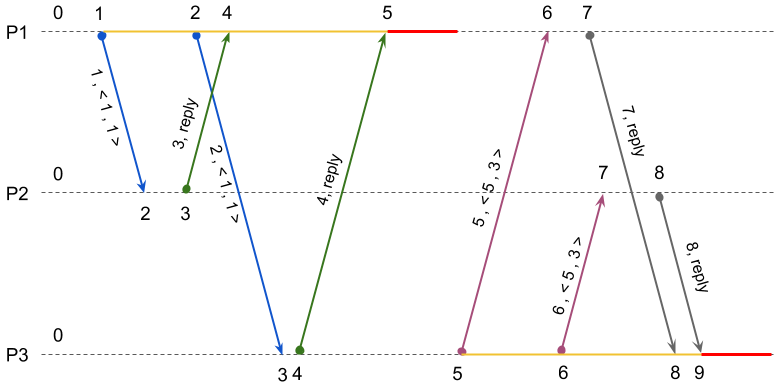
\includegraphics[scale=0.3]{imagens/ex1.png}}
\caption{Funcionamento esperado para a tarefa com 3 processos.}.
\label{ex1}
\end{figure}

	Foi simulada essa situação acima com o código implementado no laboratório, tendo os resultados apresentados nas Figuras de \ref{ex1-proc1-clean} a \ref{ex1-shared-clean}. Na simulação, ao invés de o P3 fazer a requisição, é o P2 a faz, mas isso não prejudica o teste.
	
\begin{figure}[H]
\centering
\centerline{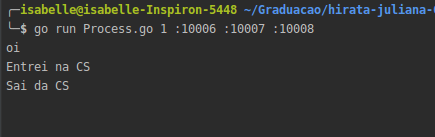
\includegraphics[scale=0.5]{imagens/ex1-proc1-clean.png}}
\caption{Exemplo do funcionamento da tarefa com 3 processos. Tela do processo 1.}.
\label{ex1-proc1-clean}
\end{figure}

\begin{figure}[H]
\centering
\centerline{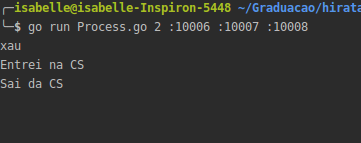
\includegraphics[scale=0.5]{imagens/ex1-proc2-clean.png}}
\caption{Exemplo do funcionamento da tarefa com 3 processos. Tela do processo 2.}.
\label{ex1-proc2-clean}
\end{figure}

\begin{figure}[H]
\centering
\centerline{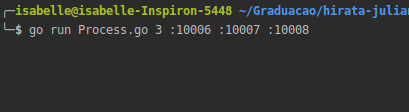
\includegraphics[scale=0.5]{imagens/ex1-proc3-clean.png}}
\caption{Exemplo do funcionamento da tarefa com 3 processos. Tela do processo 3.}.
\label{ex1-proc3-clean}
\end{figure}

\begin{figure}[H]
\centering
\centerline{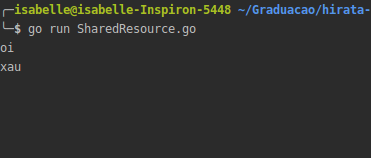
\includegraphics[scale=0.5]{imagens/ex1-shared-clean.png}}
\caption{Exemplo do funcionamento da tarefa com 3 processos. Tela do SharedResource.}.
\label{ex1-shared-clean}
\end{figure}
	
	A fim de entender melhor cada estágio do funcionamento, foram realizados os mesmos testes novamente, agora com prints de debug. Dessa forma, esses resultados estão apresentados nas Figuras de \ref{ex1-proc1} a \ref{ex1-shared}.
	
\begin{figure}[H]
\centering
\centerline{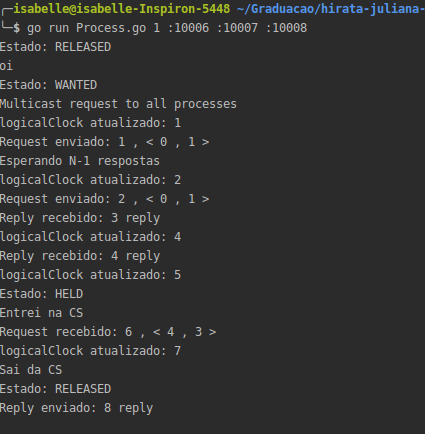
\includegraphics[scale=0.5]{imagens/ex1-proc1.png}}
\caption{Exemplo do funcionamento da tarefa com 3 processos. Tela do processo 1.}.
\label{ex1-proc1}
\end{figure}

\begin{figure}[H]
\centering
\centerline{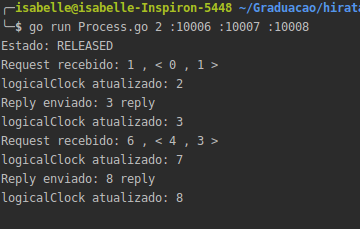
\includegraphics[scale=0.5]{imagens/ex1-proc2.png}}
\caption{Exemplo do funcionamento da tarefa com 3 processos. Tela do processo 2.}.
\label{ex1-proc2}
\end{figure}

\begin{figure}[H]
\centering
\centerline{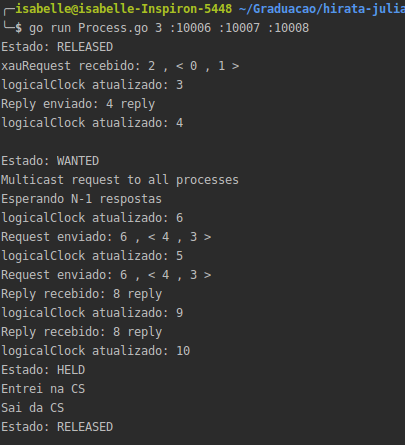
\includegraphics[scale=0.5]{imagens/ex1-proc3.png}}
\caption{Exemplo do funcionamento da tarefa com 3 processos. Tela do processo 3.}.
\label{ex1-proc3}
\end{figure}

\begin{figure}[H]
\centering
\centerline{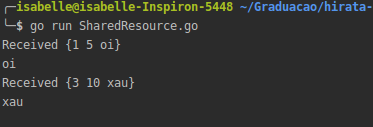
\includegraphics[scale=0.5]{imagens/ex1-shared.png}}
\caption{Exemplo do funcionamento da tarefa com 3 processos. Tela do SharedResource.}.
\label{ex1-shared}
\end{figure}

	Como esses resultados foram condizentes com os resultados esperados, leva-se a perceber que a implementação da Tarefa foi feita corretamente. Mas, antes de concluir-se algo, foi-se realizado um segundo teste.

\subsection{Teste 2}

	Este foi o caso com processos solicitando a CS "simultaneamente", sugerido no roteiro do laboratório. O esquema do resultado esperado foi apresentado na Figura \ref{ex2}.
	
	Análogo ao teste 1, na Figura \ref{ex2}, para P1, as setas azuis representam requests e as verdes, replies; e para P4, essa setas são rosas e cinzas, respectivamente. Nos requests, a mensagem enviada também é da forma "\textit{relógio lógico, < timestamp, id >}"; assim como no reply, que a forma também é "\textit{relógio lógico, 'reply'}". Além disso, nesse caso também a linha amarela representa o processo no estado WANTED; e a linha vermelha, no estado HELD, ou seja, na CS.

\begin{figure}[H]
\centering
\centerline{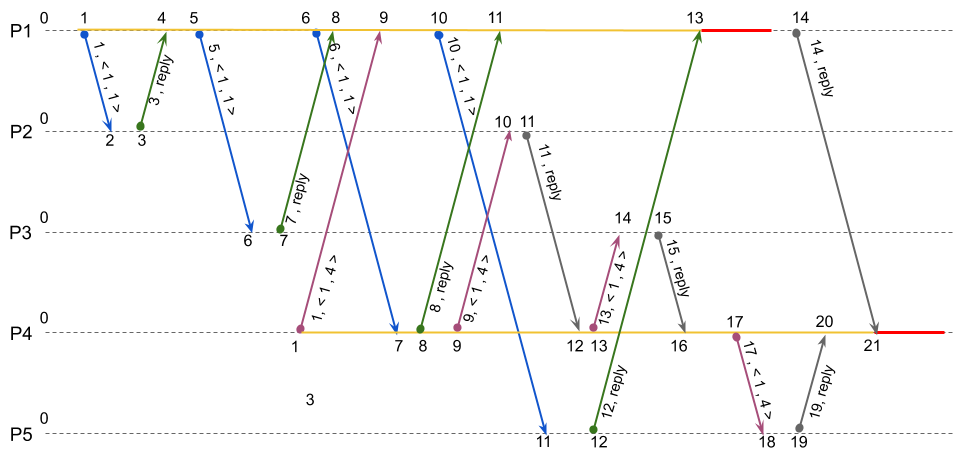
\includegraphics[scale=0.25]{imagens/ex2.png}}
\caption{Funcionamento esperado para a tarefa para 5 processos.}.
\label{ex2}
\end{figure}

	Foi simulada essa situação acima com o código implementado no laboratório, tendo os resultados apresentados nas Figuras de \ref{ex2-proc1-clean} a \ref{ex2-shared-clean}. Durante o período na CS, também foi digitado mensagens no terminal dos processos, para que se verifisse o funcionamento da validação da mensagem. Assim, para essas mensagens, foi dado o feedback de mensagem inválida.

\begin{figure}[H]
\centering
\centerline{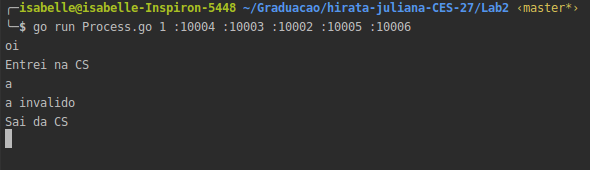
\includegraphics[scale=0.4]{imagens/ex2-proc1-clean.png}}
\caption{Exemplo do funcionamento da tarefa com 5 processos. Tela do processo 1.}.
\label{ex2-proc1-clean}
\end{figure}

\begin{figure}[H]
\centering
\centerline{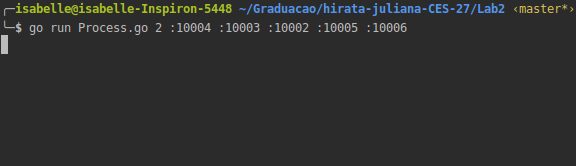
\includegraphics[scale=0.4]{imagens/ex2-proc2-clean.png}}
\caption{Exemplo do funcionamento da tarefa com 5 processos. Tela do processo 2.}.
\label{ex2-proc2-clean}
\end{figure}

\begin{figure}[H]
\centering
\centerline{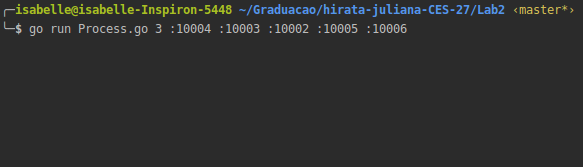
\includegraphics[scale=0.4]{imagens/ex2-proc3-clean.png}}
\caption{Exemplo do funcionamento da tarefa com 5 processos. Tela do processo 3.}.
\label{ex2-proc3-clean}
\end{figure}

\begin{figure}[H]
\centering
\centerline{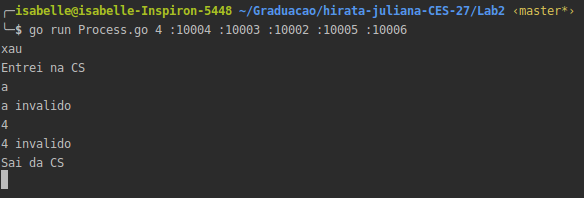
\includegraphics[scale=0.4]{imagens/ex2-proc4-clean.png}}
\caption{Exemplo do funcionamento da tarefa com 5 processos. Tela do processo 4.}.
\label{ex2-proc4-clean}
\end{figure}

\begin{figure}[H]
\centering
\centerline{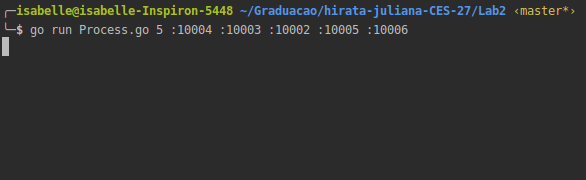
\includegraphics[scale=0.4]{imagens/ex2-proc5-clean.png}}
\caption{Exemplo do funcionamento da tarefa com 5 processos. Tela do processo 5.}.
\label{ex2-proc5-clean}
\end{figure}

\begin{figure}[H]
\centering
\centerline{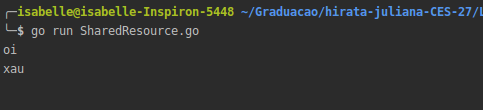
\includegraphics[scale=0.5]{imagens/ex2-shared-clean.png}}
\caption{Exemplo do funcionamento da tarefa com 5 processos. Tela do SharedResource.}.
\label{ex2-shared-clean}
\end{figure}

	A fim de entender melhor cada estágio do funcionamento, foram realizados os mesmos testes novamente, agora com prints de debug. Dessa forma, esses resultados estão apresentados nas Figuras de \ref{ex2-proc1} a \ref{ex2-shared}. Como é difícil simular com exatidão os instantes dos envios de request dos processos simultaneamente, foi feito da seguinte forma: o processo P4 entra no estado WANTED durante o estado HELD do processo P1. Isso é um pouco diferente do apresentado na Figura \ref{ex2}, mas não prejudica os testes. Contudo, isso altera um pouco a ordem dos envios de mensagens, e, consequentemente, os valores relógios lógicos.

\begin{figure}[H]
\centering
\centerline{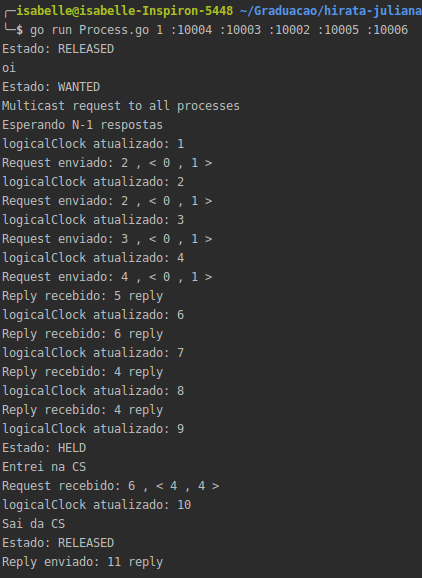
\includegraphics[scale=0.4]{imagens/ex2-proc1.png}}
\caption{Exemplo do funcionamento da tarefa com 5 processos. Tela do processo 1.}.
\label{ex2-proc1}
\end{figure}

\begin{figure}[H]
\centering
\centerline{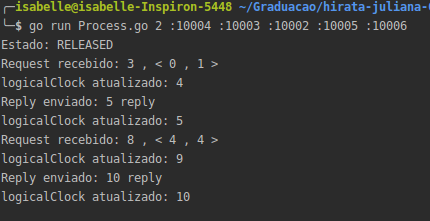
\includegraphics[scale=0.4]{imagens/ex2-proc2.png}}
\caption{Exemplo do funcionamento da tarefa com 5 processos. Tela do processo 2.}.
\label{ex2-proc2}
\end{figure}

\begin{figure}[H]
\centering
\centerline{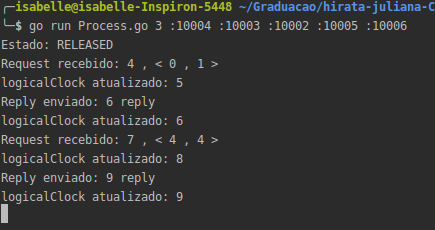
\includegraphics[scale=0.4]{imagens/ex2-proc3.png}}
\caption{Exemplo do funcionamento da tarefa com 5 processos. Tela do processo 3.}.
\label{ex2-proc3}
\end{figure}

\begin{figure}[H]
\centering
\centerline{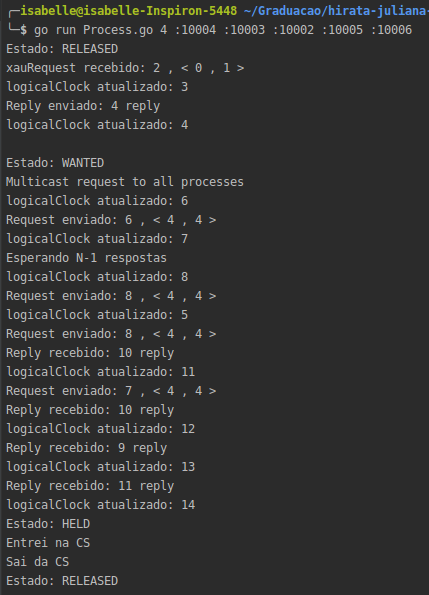
\includegraphics[scale=0.4]{imagens/ex2-proc4.png}}
\caption{Exemplo do funcionamento da tarefa com 5 processos. Tela do processo 4.}.
\label{ex2-proc4}
\end{figure}

\begin{figure}[H]
\centering
\centerline{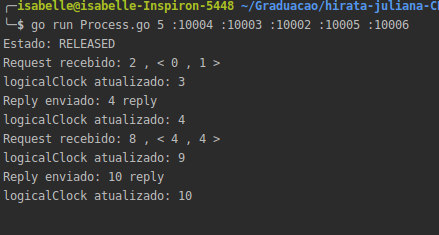
\includegraphics[scale=0.4]{imagens/ex2-proc5.png}}
\caption{Exemplo do funcionamento da tarefa com 5 processos. Tela do processo 5.}.
\label{ex2-proc5}
\end{figure}

\begin{figure}[H]
\centering
\centerline{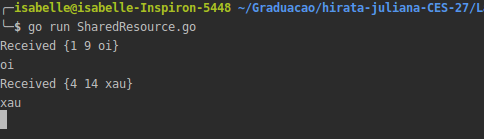
\includegraphics[scale=0.5]{imagens/ex2-shared.png}}
\caption{Exemplo do funcionamento da tarefa com 5 processos. Tela do SharedResource.}.
\label{ex2-shared}
\end{figure}
	
	Como esses resultados também foram condizentes com os resultados esperados, conclui-se que a implementação da Tarefa foi feita corretamente.
	
%\begin{thebibliography}{00}
%\bibitem{roteiro} M. Maximo, ``Roteiro: Laboratório 12 - Deep Q-Learning''. Instituto Tecnológico de Aeronáutica, Departamento de Computação. CT-213, 2019.

%\bibitem{roteiro8} M. Maximo, ``Roteiro: Laboratório 8 - Imitation Learning com Keras''. Instituto Tecnológico de Aeronáutica, Departamento de Computação. CT-213, 2019.

%\bibitem{roteiro12} M. Maximo, ``Roteiro: Laboratório 12 - Aprendizado por Reforço Livre de Modelo''. Instituto Tecnológico de Aeronáutica, Departamento de Computação. CT-213, 2019.

%\end{thebibliography}

\end{document}
